\newpage
\part{Misura della lunghezza d'onda di un laser HE-NE } \label{part:Ottica_1A}
\section{finalità}
Lo scopo di questa sezione è la misura della lunghezza d'onda,$\lambda$,di 
un laser HE-NE attraverso lo studio delle figure di diffrazione prodotte 
dal reticolo.
\section{Strumentazione}
La strumentazione impiegata nella prima parte dell'esperienza consta di:
\begin{list}{$\cdot$}{}
\item \textbf{un calibro ventesimale}, del quale abbiamo impiegato la scala gradata del righello come reticolo
di diffrazione  (passo reticolare $1$ 
$[mm]$)%non ricordo con precisione.
\item \textbf{un laser HE-NE}, quale sorgente del fascio di radiazione,di ci vogliamo calcolare la lunghezza 
d'onda.
\item \textbf{uno specchio},col quale orientare il fascio emesso dal laser.
\item \textbf{uno schermo} ove vedere la diffrazione prodotta dal reticolo.
\item \textbf{un metro a nastro},risoluzione $1$ $[cm]$,col quale misurare la distanza tra il reticolo di 
diffrazione e lo schermo.
\item \textbf{un righello},risoluzione $1$ $[mm]$ per misurare l'altezza dei vari spot 
luminosi emesso sullo schermo.

\end{list}
\bigskip


\begin{figure} [!h]
	\centering
	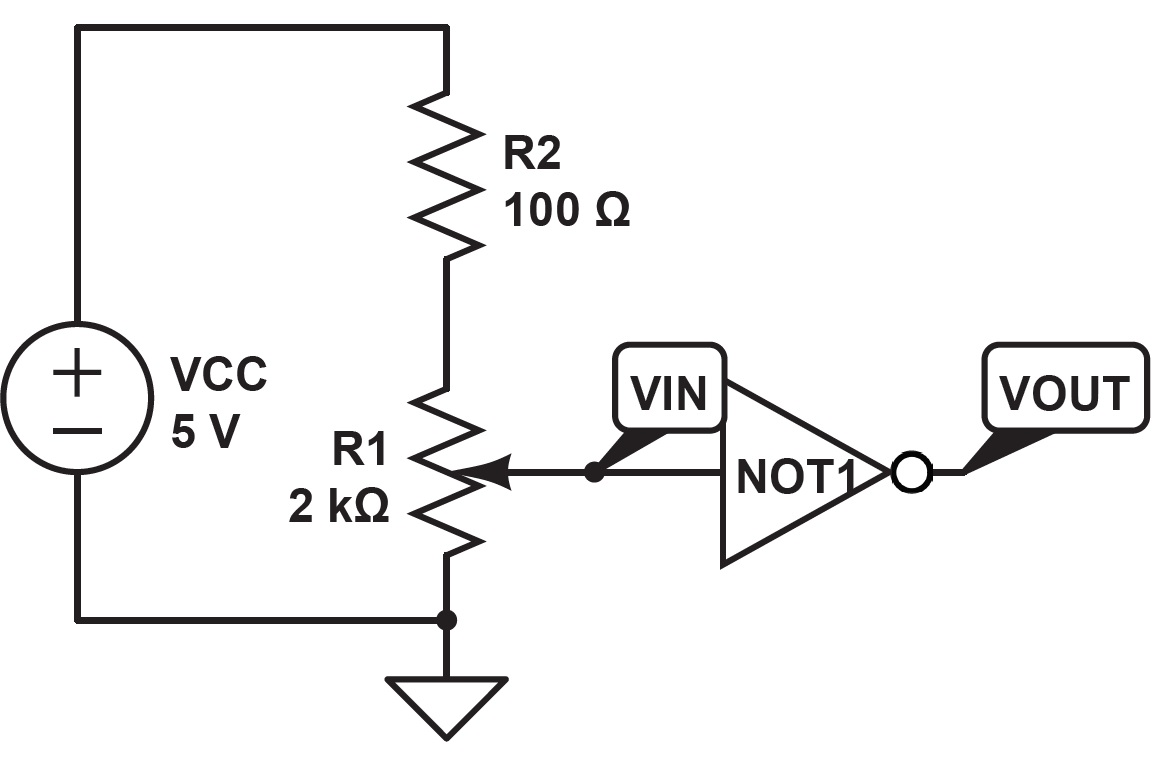
\includegraphics[width=0.9\textwidth]{./pictures/immagine1}
	\caption{Schema dell'apparato impiegato per la misura $\Lambda$.}
	\label{fig:schema_appar}
\end{figure}
Si riporta in \textbf{figura \ref{fig:schema_appar} }uno schema dell'apparato sperimentale impiegato. 